\documentclass{article}
\usepackage{graphicx}
\usepackage{bm}
\usepackage{amsmath}
\usepackage{amssymb}
\usepackage[toc,page]{appendix}
\usepackage{listings}
\usepackage{color}
\usepackage[margin=1.0in]{geometry}
\usepackage{fancyhdr}


%\numberwithin{equation}{subsection}

\definecolor{mygreen}{rgb}{0,0.6,0}
\definecolor{mygray}{rgb}{0.5,0.5,0.5}
\definecolor{mymauve}{rgb}{0.58,0,0.82}

\lstset{ %
  backgroundcolor=\color{white},   % choose the background color; you must add \usepackage{color} or \usepackage{xcolor}
  basicstyle=\footnotesize,        % the size of the fonts that are used for the code
  breakatwhitespace=false,         % sets if automatic breaks should only happen at whitespace
  breaklines=true,                 % sets automatic line breaking
  captionpos=b,                    % sets the caption-position to bottom
  commentstyle=\color{mygreen},    % comment style
  deletekeywords={...},            % if you want to delete keywords from the given language
  escapeinside={\%*}{*)},          % if you want to add LaTeX within your code
  extendedchars=true,              % lets you use non-ASCII characters; for 8-bits encodings only, does not work with UTF-8
  frame=single,	                   % adds a frame around the code
  keepspaces=true,                 % keeps spaces in text, useful for keeping indentation of code (possibly needs columns=flexible)
  keywordstyle=\color{blue},       % keyword style
  language=Octave,                 % the language of the code
  otherkeywords={*,...},            % if you want to add more keywords to the set
  numbers=left,                    % where to put the line-numbers; possible values are (none, left, right)
  numbersep=5pt,                   % how far the line-numbers are from the code
  numberstyle=\tiny\color{mygray}, % the style that is used for the line-numbers
  rulecolor=\color{black},         % if not set, the frame-color may be changed on line-breaks within not-black text (e.g. comments (green here))
  showspaces=false,                % show spaces everywhere adding particular underscores; it overrides 'showstringspaces'
  showstringspaces=false,          % underline spaces within strings only
  showtabs=false,                  % show tabs within strings adding particular underscores
  stepnumber=2,                    % the step between two line-numbers. If it's 1, each line will be numbered
  stringstyle=\color{mymauve},     % string literal style
  tabsize=2,	                   % sets default tabsize to 2 spaces
  title=\lstname                   % show the filename of files included with \lstinputlisting; also try caption instead of title
}

\pagestyle{fancy}
\fancyhf{}
\rhead{Preliminary Proposal}
\lhead{COMP SCI 6401 SP2016}
%\rfoot{Page \thepage}

\renewcommand{\thesection}{\Alph{section}}

\begin{document}

\title{Title}
\author{Edward Norris}



%\maketitle
%\thispagestyle{fancy}

%\begin{abstract}
%The abstract text goes here.
%\end{abstract}

%\tableofcontents

\section{Project Summary}\label{sec:A}

\subsection{Name and degree program}\label{sec:a1}

Edward Norris, PhD in Nuclear Engineering

\subsection{Project title}\label{sec:a2}
An Evolutionary Algorithm for Online Spatial Discretization Optimization

\subsection{Project description}\label{sec:a3}

Ionizing radiation is used extensively in many fields such as medicine, power production, and industrial non-invasive interrogation, however, utilization of such radiation poses a health concern to the surrounding populace. Engineering simulations are critical in determining the exposure to individuals in order to mitigate risks and ensure that proper protective measures are in place. However, these simulations are very time consuming, therefore, a two phase scheme is used. First, the model is simulated with a deterministic method utilizing a coarse spatial refinement mesh. This results in biasing parameters for the second phase, a high fidelity Monte Carlo calculation of exposure.

The success of the deterministic simulation in producing biasing parameters to accelerate the Monte Carlo code is highly dependent on the spatial discretization parameters selected. Unfortunately, selection of optimal parameters is very difficult and are typically tuned via experts. Therefore, an evolutionary algorithm is proposed to perform the spatial discretization refinement. Evolutionary algorithms have shown promising results in similar engineering simulations for parameter tuning including other spatial discretization tuning.

The primary drawback of utilization of an evolutionary algorithm in practical application is that each fitness evaluation necessitates a fresh start of the Monte Carlo simulation, increasing runtime untenably. However, a unique property of the two phase simulation scheme presented is that the accelerating simulation does not impact the value of the final solution, only the convergence rate. Therefore, this work proposes to evolve discretization parameters online with respect to the Monte Carlo simulation. A single Monte Carlo simulation will continuously run and spatial discretizations will be swapped out at run-time. The statistical contribution from the current deterministic simulation can be calculated for the fitness function. Further, within the online framework, each discretization in the population can be evaluated until its fitness is known only to within some statistical threshold of other members of the population. This allows pruning of poor solutions through early termination.


\subsection{Intellectual merit}\label{sec:a4}

The current state of the art in spatial discretization selection (specifically adaptive mesh refinement) utilizes octrees in 3D space. However, an octree mesh refinement is not applicable to the type of deterministic simulation used to accelerate the Monte Carlo code of interest. This necessitates development of a new representation of the spatial domain. Instead of a single octree population, three segment tree populatioins will be co-evolved using cooperative co-evolution. Novel mutation and recombination operators will have to be constructed to operate on segment trees instead of octrees.

\subsection{Societal benefit}\label{sec:a5}

Implementation of an evolutionary algorithm to accelerate generation of biasing parameters in a deterministic code for Monte Carlo codes will greatly enhance engineers ability to rapidly verify the safety of nuclear systems. Accurate simulations enable the dose to individual members of the public to be estimated so that systems can be optimized in order to reduce the levels of ionizing radiation reaching individuals, hence reducing the health impact such radiation imposes.

Further, benefits can be extended to any field that couple a non-stoichastic simulation technique to generate biasing parameters for a Monte Carlo code. Such simulation systems are very prevalent in fluid dynamics, physics, heat transfer, and many other engineering fields.

Application outside NE?

\section{Project Narrative}\label{sec:b}

\subsection{Introduction}\label{sec:b1}

Monte Carlo simulations require detailed knowledge of the geometry of a system as well as what type of radiation is emitted and from where. With this information, a Monte Carlo simulation can calculate the dose to a person at a particular location due to the radioactive sources. However, in deep shielding problems, in which a strong source is attenuated (reduced in strength) greatly, the statistical uncertainty 

The analog Monte Carlo (so called due to it being directly analogous the the physical transport process) is very slow. 

The figure of merit (FOM) is a metric used to compare the overall performance of two simulations. The FOM gives a directly comparable measure of performance for any two simulations as long as the physical problem being solved does not change and the computation hardware the two simulations were run on are identical. The FOM is defined in Eq. \ref{eq:fom} where $T$ is the wall clock runtime of the simulation and $R$ is the estimated relative uncertainty of the output.

\begin{equation} \label{eq:fom}
FOM = \frac{1}{T R^2}
\end{equation}

In important regions many samples of low weight
are tracked, while in unimportant regions few samples of high weight are tracked. A weight adjustment is made to ensure that the problem solution remains unbiased.

The weight windows are used for particle rouletting and splitting. When a particle of weight $w_p$ moves into a region of weight $w_R$ that is higher than the particles weight, it may be split into multiple particles, each of the higher weight. Conversely, if the particle moves into a region of lower weight than itself, there is a chance it will be killed; surviving particles have their weight updated to the lower weight. Between these two biasing techniques, particles that have low probability of reaching a area of interest can be killed, reducing simulation time, and other particles can artificially be propogated through a highly attenuating medium.

However, the production of accurate weight window meshes remains difficult. To remedy this, the adjoint transport calculation is made. Rather than tracking particles forward through time as they traverse space and building a mesh of dose values, the adjoint solution tracks particles backward from an object of interest and builds a mesh of influence on the region of interest. This mesh is then used directly as the weight window map.

One such solver is AutomateD VAriance NT Generator (ADVANTG) which is a code packaged developed at Oak Ridge National Lab specifically to produce weight window meshes for MCNP. However, it is up to the user to provide a spatial discretization for the weight window mesh on which the adjoint solution will be solved.

Justify use of an EA

\subsection{Related work}\label{sec:b2}

It's all good!

\subsection{Proposed research}\label{sec:b3}

Optimization of the spatial discretization for the ADVANTG code is proposed to be evolved by an evolutionary algorithm. The spatial discretization will be optimized online with respect to the Monte Carlo simulation. 

As reiterated, the current state of the art in mesh optimization uses 

\subsection{Qualifications and resources}\label{sec:b4}

The PI is a PhD student in nuclear engineering with over five years of experience with MCNP and whose research work involves usage of both MCNP and ADVANTG on a daily basis.

The PI has access to a desktop computer representative of the target platform. While running the optimization algorithm on a cluster or similiar high performance system would be preferable, there are strigent export control issues that prevent running MCNP on general computing clusters.

\subsection{Tentative work plan}\label{sec:b5}

Yeah, about that too...

\section{References}\label{sec:c}

They exist.

\begin{equation} \label{eq_boltz_t_dep}
\begin{split}
	&\left[ \frac{1}{v(E)} \frac{\partial}{\partial t} + \hat{\Omega} \cdot \nabla + \Sigma_t(\boldsymbol{r}, E, t) \right]
	\psi(\boldsymbol{r}, E, \hat{\Omega}, t) = \\
	&\int_{4 \pi} \int_0^\infty \Sigma_s(\boldsymbol{r}, E' \rightarrow E, \hat{\Omega}' \rightarrow \hat{\Omega}, t) \psi(\boldsymbol{r}, E', \hat{\Omega}', t) dE' d\hat{\Omega}' + S(\boldsymbol{r}, E, \hat{\Omega}, t)
\end{split}
\end{equation}

However, we are typically not concerned with the transient case in medical diagnostic imaging. We are more interested in the steady state case. The time independent form of Eq. \ref{eq_boltz_t_dep} is written as

\begin{equation} \label{eq_boltz}
\begin{split}
	&\left[ \hat{\Omega} \cdot \nabla + \Sigma_t(\boldsymbol{r}, E) \right]
	\psi(\boldsymbol{r}, E, \hat{\Omega}) = \\
	&\int_{4 \pi} \int_0^\infty \Sigma_s(\boldsymbol{r}, E' \rightarrow E, \hat{\Omega}' \rightarrow \hat{\Omega}) \psi(\boldsymbol{r}, E', \hat{\Omega}') dE' d\hat{\Omega}' + S(\boldsymbol{r}, E, \hat{\Omega})
\end{split}
\end{equation}

\subsection{Harmonic Approximation}
Equation \ref{eq_boltz} has a number of terms that cannot be solved directly. Instead, some numerical approximation must be used. The macroscopic scattering cross section, $\Sigma_s$ is typically expanded with a Legendre polynomial (for more information of Legendre polynomials, refer to Section \ref{sec_legendre}). The expansion is as follows:

\begin{equation} \label{eq_sigma_expansion}
\Sigma_s(\boldsymbol{r}, E' \rightarrow E, \hat{\Omega}' \rightarrow \hat{\Omega}) \approx \sum_{l=0}^L \frac{2l+1}{4 \pi} \Sigma_{s,l}(\boldsymbol{r}, E' \rightarrow E) P_l(\hat{\Omega}' \rightarrow \hat{\Omega})
\end{equation}

where $\Sigma_{s,l}$ is the expansion coefficients termed the "scattering moments." The Legendre polynomials $P_l(\hat{\Omega}' \rightarrow \hat{\Omega}$ are defined as

\begin{equation} \label{eq_harmonic}
P_l(\hat{\Omega}' \rightarrow \hat{\Omega}) = \frac{1}{2l+1}\sum_{m=-l}^l Y_{l,m}^*(\hat{\Omega}')Y_{l,m}(\hat{\Omega})
\end{equation}

The angular fluence ($\phi$) is also expanded as

\begin{equation}
\phi(\boldsymbol{r}, E', \hat{\Omega}') \approx \sum_{l=0}^L \sum_{m=-l}^l
\phi_{lm}(\boldsymbol{r}, E')Y_{lm}(\hat{\Omega}')
\end{equation}

\noindent
A source term suitable for numeric integration is then

\begin{equation}\label{eq_harmonic_simp1}
\begin{split}
\int_0^\infty dE' \int_{4 \pi} d\hat{\Omega}' \Sigma_s(\boldsymbol{r}, E' \rightarrow E, \hat{\Omega}' \rightarrow \hat{\Omega}) \phi(\boldsymbol{r}, E', \hat{\Omega}')
\approx \\
 \sum_{l=0}^L \frac{2l+1}{4 \pi} \sum_{m=-l}^l \Sigma_{s,l}^{gg'}\phi_{i,j,k,lm}^{g'}Y_{l,m}(\hat{\Omega}_n)
\end{split}
\end{equation}

Finally, substituting Eqs. \ref{eq_harmonic_simp1} and <> into <>, we arrive at

\begin{equation}\label{eq_discretized}
\begin{split}
\hat{\Omega}_n \cdot \nabla\psi_{i,j,k,n}^g + \sigma_{i,j,k}^g \psi_{i,j,k,n}^g = \\
\sum_{g' = 0}^G \sum_{l=0}^L \frac{2l+1}{4 \pi} \sum_{m=-l}^l \sigma_{s,l}^{g,g'}\psi_{i,j,k,l,m}^{g'}Y_{l,m}(\hat{\Omega}_n) + \frac{1}{4 \pi}q_{i,j,k}^g
\end{split}
\end{equation}

We can calculate the scalar flux as

\begin{equation}
\phi_{i,j,k}^g = \sum_{n=1}^{|\Omega|} w_n \psi_{i,j,k,n}^g
\end{equation}

\subsection{Discretization}
The continuous Boltzmann Equation Approximation has to be discretized in all dimensions to run on a computer.

The gradient of $\psi$ is calculated as

\begin{equation}
\nabla \psi_{i,j,k,n}^g \approx
\left\langle  
\frac{\psi_{i+1,j,k}^g - \psi_{i-1,j,k}^g}{\Delta x},
\frac{\psi_{i,j+1,k}^g - \psi_{i,j-1,k}^g}{\Delta y},
\frac{\psi_{i,j,k+1}^g - \psi_{i,j,k-1}^g}{\Delta z}
\right\rangle
\end{equation}

There are six faces on each parallelpiped with normals $<\pm 1, 0, 0>$, $<0, \pm 1, 0>$, and $<0, 0, \pm 1>$. Taking the dot product of these normals and the evaluated gradient gives

\begin{equation}
\hat{\Omega} \cdot \nabla \psi_{i,j,k}^g \approx
2 \left(
\frac{\psi_{i+1,j,k}^g - \psi_{i-1,j,k}^g}{\Delta x} +
\frac{\psi_{i,j+1,k}^g - \psi_{i,j-1,k}^g}{\Delta y} +
\frac{\psi_{i,j,k+1}^g - \psi_{i,j,k-1}^g}{\Delta z}
\right)
\end{equation}

\begin{figure}
    \centering
    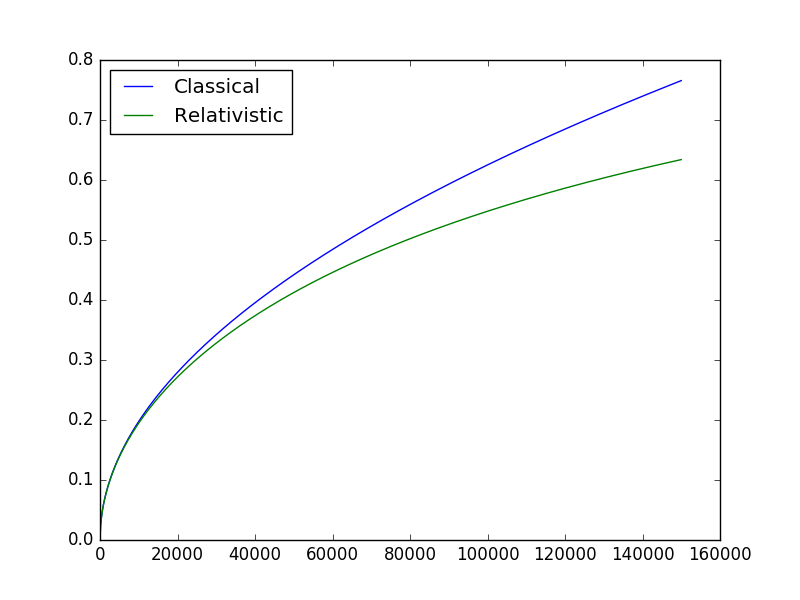
\includegraphics[width=3.0in]{test}
    \caption{Simulation Results}
    \label{simulationfigure}
\end{figure}

\section{Implementation}
At this point, we have successfully developed an algorithm that can be implemented on a computer. However, there are many challenges in actually implementing this algorithm.

\subsection{Design}
Yeah, it was designed.

\subsection{Language Selection}
Yeah, it was selected.

\subsection{Salome}
We chose to use the Salome framework for numerical pre/post-processing. Salome includes a built in geometry system and meshing capabilities.

\subsection{Framework Integration}
Yeah, it was integrated

\subsection{C++ Implementation}
Yeah, it was implemented.

\begin{lstlisting}
#include <stdio.h>
#define N 10
/* Block
 * comment */

int main()
{
    int i;

    // Line comment.
    puts("Hello world!");
    
    for (i = 0; i < N; i++)
    {
        puts("LaTeX is also great for programmers!");
    }

    return 0;
}
\end{lstlisting}

\section{MPI Implementation}
MPI stands for Message Passing Interface and is the \textit{de Facto} standard for implementing parallel algorithms across multiple physical machines.

\section{GPU Implementation}
GPU stands for Graphical Processing Unit and is a collection of SIMD (single instruction multiple data) processors. Each processor operates on its own piece of data but performs the same operation each other processor in its warp is executing.

\section{Conclusion}
Hooray! It works!

\section{Appendix}

\subsection{Laplace's Equation} \label{sec_laplace}
Many physical phenomena can be described by Poisson's Equation given below.

\begin{equation} \label{eq_poisson}
\nabla^2 f = \psi
\end{equation}

Laplace's Equation is a special form of Poisson's Equation and is given by Eq. \ref{eq_laplace}.


\begin{equation} \label{eq_laplace}
\nabla^2 f = 0
\end{equation}

Laplace's equation in cartesian coordinates expands to

\begin{equation} \label{eq_laplace_cartesian}
\nabla^2 f(x, y, z) = \frac{\partial^2 f}{\partial x^2} + \frac{\partial^2 f}{\partial y^2} + \frac{\partial^2 f}{\partial z^2} = 0
\end{equation}

In cylindrical coordinates
\begin{equation} \label{eq_laplace_cylindrical}
\nabla^2 f(r, \phi, z) = \frac{1}{r} \frac{\partial}{\partial r}\left( r \frac{\partial f}{\partial r}\right) + \frac{1}{r^2}\frac{\partial^2 f}{\partial \phi^2} + \frac{\partial^2 f}{\partial z^2}
\end{equation}

In spherical coordinates
\begin{equation} \label{eq_laplace_spherical}
\nabla^2 f(\rho, \theta, \phi) = \frac{1}{\rho^2}\frac{\partial}{\partial \rho} \left( \rho^2 \frac{\partial f}{\partial \rho}\right) + \frac{1}{\rho^2 \sin \theta}\frac{\partial}{\partial \theta}\left( \sin \theta \frac{\partial f}{\partial \theta}\right) + \frac{1}{\rho^2 \sin^2 \theta} \frac{\partial^2 f}{\partial \phi^2}
\end{equation}

Any solution to Laplace's equation is known as a harmonic function. Further, if any two functions are a solution to Laplace's equation, then by the superposition principle, the summation of the two functions is also a solution to Laplace's equation.

Common solutions to Laplace's equation include

\begin{table}
\begin{center}
\label{tbl_laplace_solutions}
\caption{A list of solutions to Laplace's equation in different geometrical systems}
\begin{tabular}{|l|c|}
\hline
Cartesian & Exponential, Circular (a class of trig function), hyperbolic \\ \hline
Cylindrical & Bessel, Exponential, Circular \\ \hline
Spherical & Legendre polynomial, Power, Circular \\ \hline
\end{tabular}
\end{center}
\end{table}

\subsection{Legendre Polynomials} \label{sec_legendre}

Legendre polynomials are solutions to
\begin{equation}
P_n(x) = \frac{1}{2 \pi i} \oint (1-2\xi x + \xi^2)^{-1/2} \xi^{-n-1} d\xi
\end{equation}

\begin{equation}
P_n(x) = \frac{1}{2^n n!}\frac{d^n}{dx^n}(x^2-1)^n
\end{equation}

The first few such solutions are \\
$P_0(x) = 1$ \\
$P_1(x) = x$ \\
$P_2(x) = \frac{1}{2}(3x^2-1)$ \\
$P_3(x) = \frac{1}{2}(5x^3 - 3x)$ \\
$P_4(x) = \frac{1}{8}(35x^4 - 30x^2 + 3)$ \\
$P_5(x) = \frac{1}{8}(63x^5 - 70x^3 + 15x)$ \\
$P_6(x) = \frac{1}{16}(231x^6 - 315x^4 + 105x^2 - 5)$ \\

Associated Legendre polynomials are a generalization of the Legendre polynomial and solve 

\begin{equation}
P_l^m(x) = (-1)^m(1-x^2)^{m/2}\frac{d^m P_l(x)}{dx^m}
\end{equation}

Both Legendre polynomials and Associated Legendre Polynomials can be calculated using the Boost C++ library.

\subsection{Spherical Harmonic Function}

First, we assume that Laplace's equation is of the seperable form $f(\rho, \theta, \phi) = R(\rho)Y(\theta, \phi)$. Equation \ref{eq_laplace_spherical} can then be rewritten as

\begin{equation} \label{eq_spherical1}
\begin{split}
\nabla^2 f(\rho, \theta, \phi) = 
\frac{1}{\rho^2}
\frac{\partial}{\partial \rho} 
\left( \rho^2 \frac{\partial (R(\rho)Y(\theta, \phi))}{\partial \rho}\right) 
+ \\
\frac{1}{\rho^2 \sin \theta}
\frac{\partial}{\partial \theta}
\left( \sin \theta \frac{\partial (R(\rho)Y(\theta, \phi))}{\partial \theta}\right) 
+ 
\frac{1}{\rho^2 \sin^2 \theta} 
\frac{\partial^2 (R(\rho)Y(\theta, \phi))}{\partial \phi^2} = 0
\end{split}
\end{equation}

\noindent
which simplifies to
\begin{equation} \label{eq_spherical2}
\begin{split}
\frac{Y(\theta, \phi)}{\rho^2}
\frac{\partial}{\partial \rho} 
\left( \rho^2 \frac{\partial R(\rho)}{\partial \rho}\right) 
+ 
\frac{R(\rho)}{\rho^2 \sin \theta}
\frac{\partial}{\partial \theta}
\left( \sin \theta \frac{\partial Y(\theta, \phi)}{\partial \theta}\right) 
+ \\
\frac{R(\rho)}{\rho^2 \sin^2 \theta} 
\frac{\partial^2 Y(\theta, \phi)}{\partial \phi^2}
\end{split} = 0
\end{equation}

\noindent
Multiplying Eq. \ref{eq_spherical2} by $\rho^2 / (R(\rho)Y(\theta, \phi))$ yields

\begin{equation}\label{eq_spherical3}
\begin{split}
\frac{1}{R(\rho)}
\frac{\partial}{\partial \rho} 
\left( \rho^2 \frac{\partial R(\rho)}{\partial \rho}\right) 
+ 
\frac{1}{Y(\theta, \phi) \sin \theta}
\frac{\partial}{\partial \theta}
\left( \sin \theta \frac{\partial Y(\theta, \phi)}{\partial \theta}\right) 
+ \\
\frac{1}{Y(\theta, \phi) \sin^2 \theta} 
\frac{\partial^2 Y(\theta, \phi)}{\partial \phi^2} = 0
\end{split}
\end{equation}

Equation \ref{eq_spherical3} can be split into two parts, a function of $\rho$ alone and a component that is a function of $\theta$ and $\phi$ alone. The component that is a function of $\theta$ and $\phi$ can be moved to the other side of the equation. Since two functions of different variables are equal, they must each be equal to some constant, $\lambda$. Therefore, Eq. \ref{eq_spherical3} can be rewritten as two equations:

\begin{equation}\label{eq_spherical_r}
\frac{1}{R(\rho)}
\frac{\partial}{\partial \rho} 
\left( \rho^2 \frac{\partial R(\rho)}{\partial \rho}\right) = \lambda
\end{equation}

\begin{equation}\label{eq_spherical_tp}
\frac{1}{Y(\theta, \phi) \sin \theta}
\frac{\partial}{\partial \theta}
\left( \sin \theta \frac{\partial Y(\theta, \phi)}{\partial \theta}\right) 
+ \\
\frac{1}{Y(\theta, \phi) \sin^2 \theta} 
\frac{\partial^2 Y(\theta, \phi)}{\partial \phi^2} = -\lambda
\end{equation}

$Y(\theta, \phi)$ can be further seperated into $Y(\theta, \phi) = \Theta(\theta)\Phi(\phi)$ which produces

\begin{equation}\label{eq_spherical_y}
\begin{split}
\frac{1}{\Theta(\theta)\Phi(\phi) \sin \theta}
\frac{\partial}{\partial \theta}
\left( \sin \theta \frac{\partial (\Theta(\theta)\Phi(\phi))}{\partial \theta}\right) 
+ \\
\frac{1}{\Theta(\theta)\Phi(\phi) \sin^2 \theta} 
\frac{\partial^2 (\Theta(\theta)\Phi(\phi))}{\partial \phi^2} = -\lambda
\end{split}
\end{equation}

\noindent
which simplifies to

\begin{equation}\label{eq_spherical_y2}
\begin{split}
\frac{1}{\Theta(\theta) \sin \theta}
\frac{\partial}{\partial \theta}
\left( \sin \theta \frac{\partial \Theta(\theta)}{\partial \theta}\right) 
+ 
\frac{1}{\Phi(\phi) \sin^2 \theta} 
\frac{\partial^2 \Phi(\phi)}{\partial \phi^2} = -\lambda
\end{split}
\end{equation}

Multiplying Eq. \ref{eq_spherical_y2} by $\sin^2(\theta)$ and rearranging yields

\begin{equation}\label{eq_spherical_y3}
\begin{split}
\frac{\sin \theta}{\Theta(\theta)}
\frac{\partial}{\partial \theta}
\left( \sin \theta \frac{\partial \Theta(\theta)}{\partial \theta}\right) 
+ \lambda \sin \theta
 = \frac{-1}{\Phi(\phi)} 
\frac{\partial^2 \Phi(\phi)}{\partial \phi^2}
\end{split}
\end{equation}

As before, each side of Eq. \ref{eq_spherical_y3} is a function of a single variable, therefore, both sides are equal to some constant. In this case, we select $m^2$ to be  the constant variable. The produces

\begin{equation}\label{eq_spherical_t}
\begin{split}
\frac{\sin \theta}{\Theta(\theta)}
\frac{\partial}{\partial \theta}
\left( \sin \theta \frac{\partial \Theta(\theta)}{\partial \theta}\right) 
+ \lambda \sin \theta
 = m^2
\end{split}
\end{equation}

\begin{equation}\label{eq_spherical_p}
\begin{split}
\frac{1}{\Phi(\phi)} 
\frac{\partial^2 \Phi(\phi)}{\partial \phi^2} = -m^2
\end{split}
\end{equation}

Combining Eq. \ref{eq_spherical_r}, \ref{eq_spherical_t}, and \ref{eq_spherical_p} Laplace's equation in sperical coordinates can be expressed in a fully seperated form as

\begin{equation}\label{eq_spherical_sep}
\begin{split}
\frac{1}{R(\rho)}
\frac{\partial}{\partial \rho} 
\left( \rho^2 \frac{\partial R(\rho)}{\partial \rho}\right) 
&= \lambda \\
\frac{\sin \theta}{\Theta(\theta)}
\frac{\partial}{\partial \theta}
\left( \sin \theta \frac{\partial \Theta(\theta)}{\partial \theta}\right) 
+ \lambda \sin \theta
&= m^2 \\
\frac{1}{\Phi(\phi)} 
\frac{\partial^2 \Phi(\phi)}{\partial \phi^2}
&= -m^2
\end{split}
\end{equation}

It can be shown through a detailed anlysis that is outside the scope of this paper that $m$ and $\lambda$ must both be integers. $\lambda$ is further constrained in that the relation $\lambda = l(l+1)$ where $l \leq |m|$ and $l \in \mathbb{Z}$. Therefore, Eq. \ref{eq_spherical_sep} can be written as

\begin{equation}\label{eq_spherical_sep2}
\begin{split}
\frac{1}{R(\rho)}
\frac{\partial}{\partial \rho} 
\left( \rho^2 \frac{\partial R(\rho)}{\partial \rho}\right) 
&= l(l+1) \\
\frac{\sin \theta}{\Theta(\theta)}
\frac{\partial}{\partial \theta}
\left( \sin \theta \frac{\partial \Theta(\theta)}{\partial \theta}\right) 
+ l(l+1) \sin \theta
&= m^2 \\
\frac{1}{\Phi(\phi)} 
\frac{\partial^2 \Phi(\phi)}{\partial \phi^2}
&= -m^2 \\
& l, m \in \mathbb{Z} \\
& l \leq |m|
\end{split}
\end{equation}

% TODO
TODO - Discontinuous

It can be shown that the solution is stated

\begin{equation}
Y_l^m(\theta, \phi) = \sqrt{\frac{2l+1}{4 \pi}
\frac{(l-m)!}{(l+m)!}} P_l^m(\cos \theta) e^{im\phi}
\end{equation}

whose real part can be expanded to

\begin{equation}
Y_l^0 = \sqrt{\frac{2l+1}{4 \pi}}P_l^0(1)
\end{equation}

\begin{equation}
Y_l^{m, even} = (-1)^m\sqrt{\frac{2l+1}{2 \pi} \frac{(l-m)!}{(l+m)!}}P_l^m(\cos(m \phi))
\end{equation}

\begin{equation}
Y_l^{m,odd} = (-1)^m \sqrt{\frac{2l+1}{2 \pi} \frac{(l-m)!}{(l+m)!}}P_l^m(\sin(m \phi))
\end{equation}

\subsection{Klein-Nishina Formula}

The Klein-Nishina formula gives the differential scattering cross section of photon incident on a single free electron.

\begin{equation}\label{klein_nishina}
\frac{\partial \sigma}{\partial \Omega} = \frac{1}{2}\alpha^2 r_c^2 P(E_\gamma, \theta)^2
\left( P(E_\gamma, \theta) + P(E_\gamma, \theta)^{-1} - 1 + \cos^2(\theta) \right)
\end{equation}

\begin{equation}\label{klein_nishina2}
P(E_\gamma, \theta) = \frac{1}{1 + (\frac{E_\gamma}{m_e c^2})(1-\cos(\theta))}
\end{equation}


\noindent
where $\alpha$ is the fine structure constant ($\alpha \approx 7.2971E-3$), $r_c$ is the reduced Compton wavelength ($r_c = \hbar$)

\subsection{Numeric Integration}

\begin{equation}
\tilde{H}
\end{equation}

\end{document}